% Options for packages loaded elsewhere
\PassOptionsToPackage{unicode}{hyperref}
\PassOptionsToPackage{hyphens}{url}
%
\documentclass[
]{article}
\author{}
\date{}

\usepackage{amsmath,amssymb}
\usepackage{lmodern}
\usepackage{iftex}
\ifPDFTeX
  \usepackage[T1]{fontenc}
  \usepackage[utf8]{inputenc}
  \usepackage{textcomp} % provide euro and other symbols
\else % if luatex or xetex
  \usepackage{unicode-math}
  \defaultfontfeatures{Scale=MatchLowercase}
  \defaultfontfeatures[\rmfamily]{Ligatures=TeX,Scale=1}
\fi
% Use upquote if available, for straight quotes in verbatim environments
\IfFileExists{upquote.sty}{\usepackage{upquote}}{}
\IfFileExists{microtype.sty}{% use microtype if available
  \usepackage[]{microtype}
  \UseMicrotypeSet[protrusion]{basicmath} % disable protrusion for tt fonts
}{}
\makeatletter
\@ifundefined{KOMAClassName}{% if non-KOMA class
  \IfFileExists{parskip.sty}{%
    \usepackage{parskip}
  }{% else
    \setlength{\parindent}{0pt}
    \setlength{\parskip}{6pt plus 2pt minus 1pt}}
}{% if KOMA class
  \KOMAoptions{parskip=half}}
\makeatother
\usepackage{xcolor}
\IfFileExists{xurl.sty}{\usepackage{xurl}}{} % add URL line breaks if available
\IfFileExists{bookmark.sty}{\usepackage{bookmark}}{\usepackage{hyperref}}
\hypersetup{
  hidelinks,
  pdfcreator={LaTeX via pandoc}}
\urlstyle{same} % disable monospaced font for URLs
\usepackage{color}
\usepackage{fancyvrb}
\newcommand{\VerbBar}{|}
\newcommand{\VERB}{\Verb[commandchars=\\\{\}]}
\DefineVerbatimEnvironment{Highlighting}{Verbatim}{commandchars=\\\{\}}
% Add ',fontsize=\small' for more characters per line
\newenvironment{Shaded}{}{}
\newcommand{\AlertTok}[1]{\textcolor[rgb]{1.00,0.00,0.00}{\textbf{#1}}}
\newcommand{\AnnotationTok}[1]{\textcolor[rgb]{0.38,0.63,0.69}{\textbf{\textit{#1}}}}
\newcommand{\AttributeTok}[1]{\textcolor[rgb]{0.49,0.56,0.16}{#1}}
\newcommand{\BaseNTok}[1]{\textcolor[rgb]{0.25,0.63,0.44}{#1}}
\newcommand{\BuiltInTok}[1]{#1}
\newcommand{\CharTok}[1]{\textcolor[rgb]{0.25,0.44,0.63}{#1}}
\newcommand{\CommentTok}[1]{\textcolor[rgb]{0.38,0.63,0.69}{\textit{#1}}}
\newcommand{\CommentVarTok}[1]{\textcolor[rgb]{0.38,0.63,0.69}{\textbf{\textit{#1}}}}
\newcommand{\ConstantTok}[1]{\textcolor[rgb]{0.53,0.00,0.00}{#1}}
\newcommand{\ControlFlowTok}[1]{\textcolor[rgb]{0.00,0.44,0.13}{\textbf{#1}}}
\newcommand{\DataTypeTok}[1]{\textcolor[rgb]{0.56,0.13,0.00}{#1}}
\newcommand{\DecValTok}[1]{\textcolor[rgb]{0.25,0.63,0.44}{#1}}
\newcommand{\DocumentationTok}[1]{\textcolor[rgb]{0.73,0.13,0.13}{\textit{#1}}}
\newcommand{\ErrorTok}[1]{\textcolor[rgb]{1.00,0.00,0.00}{\textbf{#1}}}
\newcommand{\ExtensionTok}[1]{#1}
\newcommand{\FloatTok}[1]{\textcolor[rgb]{0.25,0.63,0.44}{#1}}
\newcommand{\FunctionTok}[1]{\textcolor[rgb]{0.02,0.16,0.49}{#1}}
\newcommand{\ImportTok}[1]{#1}
\newcommand{\InformationTok}[1]{\textcolor[rgb]{0.38,0.63,0.69}{\textbf{\textit{#1}}}}
\newcommand{\KeywordTok}[1]{\textcolor[rgb]{0.00,0.44,0.13}{\textbf{#1}}}
\newcommand{\NormalTok}[1]{#1}
\newcommand{\OperatorTok}[1]{\textcolor[rgb]{0.40,0.40,0.40}{#1}}
\newcommand{\OtherTok}[1]{\textcolor[rgb]{0.00,0.44,0.13}{#1}}
\newcommand{\PreprocessorTok}[1]{\textcolor[rgb]{0.74,0.48,0.00}{#1}}
\newcommand{\RegionMarkerTok}[1]{#1}
\newcommand{\SpecialCharTok}[1]{\textcolor[rgb]{0.25,0.44,0.63}{#1}}
\newcommand{\SpecialStringTok}[1]{\textcolor[rgb]{0.73,0.40,0.53}{#1}}
\newcommand{\StringTok}[1]{\textcolor[rgb]{0.25,0.44,0.63}{#1}}
\newcommand{\VariableTok}[1]{\textcolor[rgb]{0.10,0.09,0.49}{#1}}
\newcommand{\VerbatimStringTok}[1]{\textcolor[rgb]{0.25,0.44,0.63}{#1}}
\newcommand{\WarningTok}[1]{\textcolor[rgb]{0.38,0.63,0.69}{\textbf{\textit{#1}}}}
\usepackage{graphicx}
\makeatletter
\def\maxwidth{\ifdim\Gin@nat@width>\linewidth\linewidth\else\Gin@nat@width\fi}
\def\maxheight{\ifdim\Gin@nat@height>\textheight\textheight\else\Gin@nat@height\fi}
\makeatother
% Scale images if necessary, so that they will not overflow the page
% margins by default, and it is still possible to overwrite the defaults
% using explicit options in \includegraphics[width, height, ...]{}
\setkeys{Gin}{width=\maxwidth,height=\maxheight,keepaspectratio}
% Set default figure placement to htbp
\makeatletter
\def\fps@figure{htbp}
\makeatother
\setlength{\emergencystretch}{3em} % prevent overfull lines
\providecommand{\tightlist}{%
  \setlength{\itemsep}{0pt}\setlength{\parskip}{0pt}}
\setcounter{secnumdepth}{-\maxdimen} % remove section numbering
\ifLuaTeX
  \usepackage{selnolig}  % disable illegal ligatures
\fi

\begin{document}

\hypertarget{assignment-1}{%
\section{Assignment 1}\label{assignment-1}}

By Christian Mauffette Denis

\hypertarget{question-1}{%
\subsection{Question 1}\label{question-1}}

\hypertarget{a}{%
\subsubsection{a)}\label{a}}

We can use a different formula to compute the derivative using the given
points. We know that

\[f(x + \delta) = f(x) + f'(x) \delta + \frac{f''(x)}{2}\delta^2 + \frac{f'''(x)}{6}\delta^3 + \frac{f^{(4)}(x)}{24}\delta^4 + \frac{f^{(5)}(x)}{120}\delta^5 + ...  \]

\[f(x - \delta) = f(x) - f'(x) + \frac{f''(x)}{2}\delta^2 - \frac{f'''(x)}{6}\delta^3 + \frac{f^{(4)}(x)}{24}\delta^4 - \frac{f^{(5)}(x)}{120}\delta^5 + ...  \]

\[f(x + 2\delta) = f(x) + 2 f'(x) \delta + \frac{4 f''(x)}{2}\delta^2 + \frac{8 f'''(x)}{6}\delta^3 + \frac{16 f^{(4)}(x)}{24}\delta^4 + \frac{32 f^{(5)}(x)}{120}\delta^5 + ...  \]

\[f(x - 2\delta) = f(x) - 2 f'(x) \delta + \frac{4 f''(x)}{2}\delta^2 - \frac{8 f'''(x)}{6}\delta^3 + \frac{16 f^{(4)}(x)}{24}\delta^4 - \frac{32 f^{(5)}(x)}{120}\delta^5 + ...  \]

If we subtract the first two expression we get:

\[f(x + \delta) - f(x - \delta) = 2 f'(x) \delta + \frac{ 2 f'''(x)}{6}\delta^3 + \frac{2 f^{(5)}(x)}{120}\delta^5 + ...  \]

\[ = 2 f'(x) \delta + \frac{ f'''(x)}{3}\delta^3 + \frac{ f^{(5)}(x)}{60}\delta^5 + ...  \]

Now we subtract the two last expressions:

\[ f(x + 2\delta) - f(x - 2\delta) = 4 f'(x) \delta  + \frac{8 f'''(x)}{3}\delta^3 + \frac{8 f^{(5)}(x)}{15}\delta^5 + ...  \]

This means we can get rid of the 3rd order corrections by doing:

\[\frac{2}{3} \left((f(x + \delta)-f(x-\delta ))-\frac{1}{8} (f(x + 2 \delta)-f(x-2 \delta ))\right) = f'(x)\delta -\frac{1}{30} f^{(5)}(x) \delta^5 + O\left(x^6\right)\]

Hence the error term is

\[\frac{1}{30} f^{(5)}(x) \delta^4\]

And the estimate will be

\[\frac{2}{3 \delta} \left((f(x + \delta)-f(x-\delta ))-\frac{1}{8} (f(x + 2 \delta)-f(x-2 \delta ))\right)\]

\hypertarget{b}{%
\subsubsection{b)}\label{b}}

If the roundoff error is \(\epsilon\), then the error is bounded by

\[\frac{2}{3 \delta} \left(\epsilon-(-\epsilon)-\frac{1}{8} ((-\epsilon)-\epsilon)\right) + \frac{1}{30} f^{(5)}(x) \delta^4 = \text{error}\]

\[\frac{2}{3 \delta} \left(2 \epsilon-\frac{\epsilon}{4} \right) + \frac{1}{30} f^{(5)}(x) \delta^4 = \text{error}\]

\[ \frac{7\epsilon}{6 \delta}  + \frac{1}{30} f^{(5)}(x) \delta^4 = \text{error}\]

Taking the derivative with respect to \(\delta\) and setting it equal to
0 to minimize it we have:

\[ \frac{d}{d\delta} \left( \frac{7\epsilon}{6 \delta}  + \frac{1}{30} f^{(5)}(x) \delta^4 \right) = 0 \]

\[\frac{2 \delta ^3 k}{15}-\frac{7 \epsilon }{6 \delta ^2} = 0 \]

\[\implies \delta \approx \left( \frac{35 \epsilon}{4 f^{(5)}(x) } \right)^{1/5} \]

So, assuming machine precision is about \(10^{-16}\), then we have about

\[\delta \approx 10^{-16/5} \approx 10^{-3.2}\]

We can now try this with code by evaluating the given functions with our
derivative. First we create the derivative taking function.

\begin{Shaded}
\begin{Highlighting}[]
\CommentTok{\# Function to take the derivative at some point with a given step size}
\KeywordTok{def}\NormalTok{ deriv(func, x0, delta):}
    \ControlFlowTok{return} \DecValTok{2}\OperatorTok{/}\NormalTok{(}\DecValTok{3}\OperatorTok{*}\NormalTok{delta) }\OperatorTok{*}\NormalTok{ (func(x0 }\OperatorTok{+}\NormalTok{ delta) }\OperatorTok{{-}}\NormalTok{ func(x0 }\OperatorTok{{-}}\NormalTok{ delta) }\OperatorTok{{-}} \DecValTok{1}\OperatorTok{/}\DecValTok{8}\OperatorTok{*}\NormalTok{(func(x0 }\OperatorTok{+} \DecValTok{2}\OperatorTok{*}\NormalTok{delta) }\OperatorTok{{-}}\NormalTok{ func(x0 }\OperatorTok{{-}} \DecValTok{2}\OperatorTok{*}\NormalTok{delta)))}
\end{Highlighting}
\end{Shaded}

With this function, we can pick a \texttt{x0} and then scan
(logarithmically) through different \texttt{delta} values. For the
function \(e^{x}\) whose derivative is evaluated at \(x=0\), this
produces the following plot:

\begin{figure}
\centering
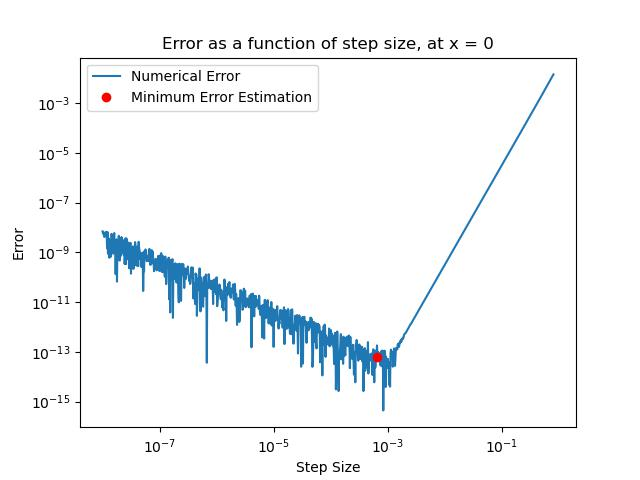
\includegraphics{figs/q1_error_plot1.jpg}
\caption{q1\_error\_plot1}
\end{figure}

We can see on it the estimated optimal error is indeed in the
\(10^{-3}\) ballpark. Also, it was assumed that the fifth derivative is
roughly of order 1, which is exactly right for our specific function,
since \(\frac{d^5}{dx^5} e^x = e^x\).

Now we can try the same procedure, but for the \(e^{0.01 x}\) function.
Again, we scan the different deltas, and produce the following plot:

\begin{figure}
\centering
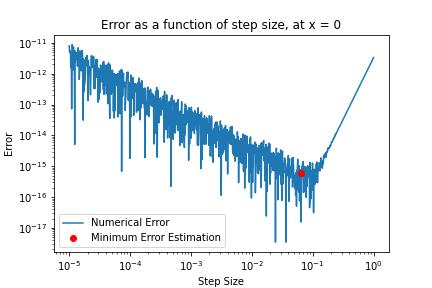
\includegraphics{figs/q1_error_plot2.jpg}
\caption{q1\_error\_plot2}
\end{figure}

For this plot the order of magnitude of the 5th derivative was in fact
significant since \(\frac{d^5}{dx^5} e^x = (0.01)^5e^x\). Hence, the
optimal step size had to be divided by \(0.01\) and after doing so, we
see that it does indeed fall roughly on the minimum of the curve for the
error.

\hypertarget{question-2}{%
\subsection{Question 2}\label{question-2}}

We now code a derivative taking function. We used the centered
derivative for that. We simply use the formula

\[\frac{f(x+\Delta x)-f(x - \Delta x)}{2 \Delta x} = f'(x)\]

However, we must pick the appropriate \(\Delta x\). If we look at the
Taylor expansion of the previous expression, we have

\[f(x + \delta) = f(x) + f'(x) \delta + \frac{f''(x)}{2}\delta^2 + \frac{f'''(x)}{6}\delta^3 + \frac{f^{(4)}(x)}{24}\delta^4 + \frac{f^{(5)}(x)}{120}\delta^5 + ...  \]

\[f(x - \delta) = f(x) - f'(x) + \frac{f''(x)}{2}\delta^2 - \frac{f'''(x)}{6}\delta^3 + \frac{f^{(4)}(x)}{24}\delta^4 - \frac{f^{(5)}(x)}{120}\delta^5 + ...  \]

\[\implies \frac{f(x+\Delta x)-f(x - \Delta x)}{2 \Delta x} = \frac{1}{2 \Delta x}\left( 2 f'(x) \Delta x + \frac{f'''(x)}{3}\Delta x^3\right) + ...\]

\[ =  f'(x)  + \frac{f'''(x)}{6}\Delta x^2 + ...\]

Hence, the error is

\[\text{error} \approx \frac{\epsilon}{\Delta x}  + \frac{f'''(x)}{6}\Delta x^2\]

If we minimize it with respect to \(\Delta x\), we have

\[\Delta x \approx \left(\frac{3 \epsilon}{f'''(x)} \right)^{1/3}\]

We will code a function that will find the 3rd derivative with a delta
value that is not optimal and then use that derivative to find the first
derivative, but this time with a delta that is quite optimal. I am
assuming that the error will be relatively small in the 3rd derivative,
hence, it should not be too much of a problem since it's only used to
roughly find the optimal value for the derivative.

We still need to find some delta to use that is not too far-fetched for
the three consecutive derivatives. In class we have seen that to
minimize the error for such a derivative prescription (central), we must
use \(\Delta x \approx 10^{-5}\), assuming second derivatives are not
too crazy and that our machine \(\epsilon\) is \(\approx 10^{-16}\).

\begin{Shaded}
\begin{Highlighting}[]

\KeywordTok{def}\NormalTok{ ndiff(fun, x, full }\OperatorTok{=} \VariableTok{False}\NormalTok{):}
    \CommentTok{\textquotesingle{}\textquotesingle{}\textquotesingle{}Function to take a derivate. Optional: can output the estimated error on the result.\textquotesingle{}\textquotesingle{}\textquotesingle{}}
    
\NormalTok{    ini\_step }\OperatorTok{=} \DecValTok{10}\OperatorTok{**{-}}\DecValTok{5} \CommentTok{\# Initial step size (for third derivative)}
    
    \CommentTok{\# Anonymous function to take derivatives}
\NormalTok{    diff\_op }\OperatorTok{=} \KeywordTok{lambda}\NormalTok{ func, x: (func(x }\OperatorTok{+}\NormalTok{ ini\_step) }\OperatorTok{{-}}\NormalTok{ func(x }\OperatorTok{{-}}\NormalTok{ ini\_step))}\OperatorTok{/}\NormalTok{(}\DecValTok{2}\OperatorTok{*}\NormalTok{ini\_step)}

\NormalTok{    deriv\_1 }\OperatorTok{=} \KeywordTok{lambda}\NormalTok{ x: diff\_op(fun, x)     }\CommentTok{\# Calculating the first derivative}
\NormalTok{    deriv\_2 }\OperatorTok{=} \KeywordTok{lambda}\NormalTok{ x: diff\_op(deriv\_1, x) }\CommentTok{\# Calculating the second derivative}
\NormalTok{    deriv\_3 }\OperatorTok{=} \KeywordTok{lambda}\NormalTok{ x: diff\_op(deriv\_1, x) }\CommentTok{\# Calculating the thirs derivative}
    
    \CommentTok{\# Optimal step size}
\NormalTok{    third\_deriv }\OperatorTok{=}\NormalTok{ deriv\_3(x)}
    \BuiltInTok{print}\NormalTok{(third\_deriv)}
\NormalTok{    opt\_step }\OperatorTok{=}\NormalTok{ (}\BuiltInTok{abs}\NormalTok{(}\DecValTok{3}\OperatorTok{*}\NormalTok{np.finfo(}\BuiltInTok{float}\NormalTok{).eps}\OperatorTok{/}\NormalTok{third\_deriv))}\OperatorTok{**}\NormalTok{(}\DecValTok{1}\OperatorTok{/}\DecValTok{3}\NormalTok{)}
    
    \CommentTok{\# Finding the derivative}
\NormalTok{    deriv }\OperatorTok{=}\NormalTok{ (fun(x }\OperatorTok{+}\NormalTok{ opt\_step) }\OperatorTok{{-}}\NormalTok{ fun(x }\OperatorTok{{-}}\NormalTok{ opt\_step))}\OperatorTok{/}\NormalTok{(}\DecValTok{2}\OperatorTok{*}\NormalTok{opt\_step)}

    \CommentTok{\# Conditional system for optional argument}
    \ControlFlowTok{if}\NormalTok{ full:}
        \CommentTok{\# Returns derivative and estimated error}
\NormalTok{        est\_err }\OperatorTok{=}\NormalTok{ np.finfo(}\BuiltInTok{float}\NormalTok{).eps}\OperatorTok{/}\NormalTok{opt\_step }\OperatorTok{+}\NormalTok{ third\_deriv}\OperatorTok{*}\NormalTok{opt\_step}\OperatorTok{**}\DecValTok{2}\OperatorTok{/}\DecValTok{6}
        \ControlFlowTok{return}\NormalTok{ np.array([deriv, est\_err])}
    
    \ControlFlowTok{elif} \KeywordTok{not}\NormalTok{ full:}
        \CommentTok{\# Returns only derivative}
        \ControlFlowTok{return}\NormalTok{ deriv}
\end{Highlighting}
\end{Shaded}

\hypertarget{question-3}{%
\subsection{Question 3}\label{question-3}}

To answer this question we create the following function

\begin{Shaded}
\begin{Highlighting}[]
\KeywordTok{def}\NormalTok{ lakeshore(V, data):}
    \CommentTok{\textquotesingle{}\textquotesingle{}\textquotesingle{}Function to interpolate the data with a cubic spline\textquotesingle{}\textquotesingle{}\textquotesingle{}}
\NormalTok{    temperatures }\OperatorTok{=}\NormalTok{ np.array([i[}\DecValTok{0}\NormalTok{] }\ControlFlowTok{for}\NormalTok{ i }\KeywordTok{in}\NormalTok{ data[::}\OperatorTok{{-}}\DecValTok{1}\NormalTok{]]) }\CommentTok{\# Making array for temperatures (from raw data)}
\NormalTok{    voltages }\OperatorTok{=}\NormalTok{ np.array([i[}\DecValTok{1}\NormalTok{] }\ControlFlowTok{for}\NormalTok{ i }\KeywordTok{in}\NormalTok{ data[::}\OperatorTok{{-}}\DecValTok{1}\NormalTok{]]) }\CommentTok{\# Making array for volatages (from raw data)}
\NormalTok{    approx\_vol\_size }\OperatorTok{=} \BuiltInTok{abs}\NormalTok{(voltages[}\DecValTok{2}\NormalTok{]}\OperatorTok{{-}}\NormalTok{voltages[}\DecValTok{1}\NormalTok{])}
    
    \CommentTok{\# First we find the interpolation}
\NormalTok{    cs }\OperatorTok{=}\NormalTok{ sci.interpolate.CubicSpline(voltages, temperatures) }\CommentTok{\# spline function}
\NormalTok{    inter\_val }\OperatorTok{=}\NormalTok{ cs(V)}

    \CommentTok{\# Now we roughly estimate the error}
\NormalTok{    lin\_spline }\OperatorTok{=}\NormalTok{ sci.interpolate.interp1d(voltages, temperatures) }\CommentTok{\# Linear interpolation}
\NormalTok{    err\_range }\OperatorTok{=}\NormalTok{ np.array(np.linspace(V}\OperatorTok{{-}}\NormalTok{approx\_vol\_size, V}\OperatorTok{+}\NormalTok{approx\_vol\_size, }\DecValTok{1000}\NormalTok{))}

\NormalTok{    approx\_error }\OperatorTok{=}\NormalTok{ np.std(}\BuiltInTok{abs}\NormalTok{(lin\_spline(err\_range) }\OperatorTok{{-}}\NormalTok{ cs(err\_range)), axis }\OperatorTok{=} \DecValTok{0}\NormalTok{)}


    \ControlFlowTok{return}\NormalTok{ inter\_val, approx\_error}
\end{Highlighting}
\end{Shaded}

This function takes as input the value(s) we want to evaluate at an
interpolated value and the raw data to create the interpolation. The
function starts by extracting arrays for the temperature and the
voltages from the raw data. From these \(x\) and \(y\) set of data, we
are able to create the interpolation. To find the error on the obtained
values, we create another interpolation, but this time linear. We look
at the difference between the linear and the cubic splined
interpolations to obtain a rough estimate for the error. This difference
should give us roughly an order of magnitude estimate of the error. The
rationale behinnd it is that the cubic spline can be ``curvier'' than
the actual data, while the linear fit is often not curvy enough, hence
the true value is hypothesized to fall within the two fit. This is where
this substraction came from.

All this is down with arrays, so the function can work with both single
value or arrays for \texttt{V}. It will return two elements, the first
is either an array or single value for the interpolated value and the
second is the rough estimate for the error (also as array or value).

The interpolation can be observed in the following plot:

\begin{figure}
\centering
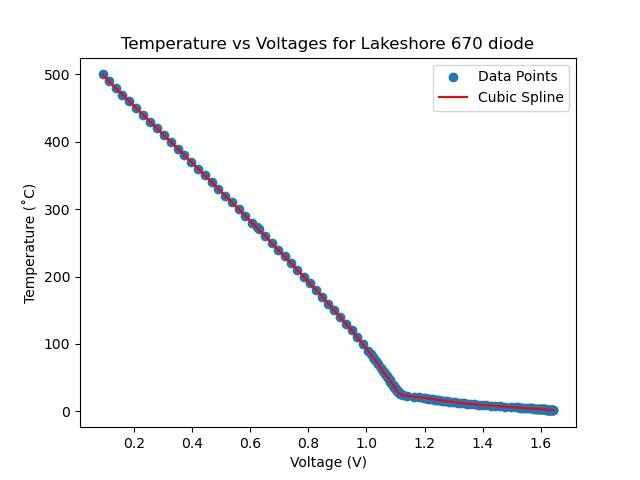
\includegraphics{figs/q3_interp_plot.jpg}
\caption{q3\_interp\_plot}
\end{figure}

\hypertarget{question-4}{%
\subsection{Question 4}\label{question-4}}

\hypertarget{cos-x}{%
\subsubsection{\texorpdfstring{\(\cos (x)\)}{\textbackslash cos (x)}}\label{cos-x}}

We create three different interpolations for samples of the \(\cos (x)\)
function.

The first is a polynomial fit of degree \(n-1\) where \(n\) is the
number of samples used. \texttt{scipy}'s \texttt{polyfit} function was
used for that.

The second interpolation scheme used was a cubic spine. Similarly to the
polynomial fit, we used \texttt{scipy}'s \texttt{polyfit}'s
\texttt{interpolate.CubicSpline} function.

\hypertarget{lorentzian}{%
\subsubsection{Lorentzian}\label{lorentzian}}

\end{document}
